% Basic US Letter document format
% by C. G. Wilson 
% modified by Morgan Fine-Morris

\documentclass[11pt]{article}
\usepackage{amsfonts}
\usepackage[pdftex]{graphicx}
\usepackage[space]{grffile}
\usepackage{caption}
\usepackage{subcaption}
\usepackage{placeins}

\usepackage{multicol}
\setlength{\columnsep}{1cm}

% \usepackage{palatino}

%%formatting
\textwidth 6.85in
\textheight 8.75in

\pagestyle{headings}
%\markright{\today, header}

\newcommand{\tsscale}{0.45}
\newcommand{\bcscale}{0.2}

\begin{document}

%%formatting
\oddsidemargin -0.22in
\evensidemargin -0.22in
\topmargin 0.05in
\topskip 0.25in
\headheight 0.05in
\headsep 0.25in

\graphicspath{{"../Data and Analysis/long TB Yan/plots/"}{"../Data and Analysis/short TB Yan/plots/"}}
%{"../Data and Analysis/long TB Yan/plots/Comparative TS Yan/"}{"../Data and Analysis/long TB Yan/plots/Comparative TS TB/"}}
%\begin{center}
%\Large{\textbf{Results}}
%\end{center}

\FloatBarrier
\section{Results}
The Yan model clearly shows a bias towards greater excitement with shorter interburst intervals, longer burst duration
Comparing time series Figures~\ref{fig:ts18} and~\ref{fig:ts42}, we can see that generally, the Yan model exhibits longer bursts with more leading-edge spikes and that around $eL$=-50, bursting becomes tonic spiking, while the TB model has shorter, tighter bursts and continues to exhibit bursting even into $eL$=-50. 

Additionally, while the TB model exhibits bursting at $eL$=-50 when $g_{NaP}$=1.8 or 2.4, the Yan model exhibits only tonic spiking when  $eL$=-50. Note, however, that even in time series containing only tonic spiking, spike density does increase and decrease periodically and the effect is more noticeable when $g_{NaP}$ is small. 

The most interesting feature visible in the time series occurs at $gnap$ = 4.2, $eL$=-55. In the Yan model, spike frequency at the start and end of a burst is visibly higher than spike frequency at the burst center, while in the TB model we see bi-modal bursting behavior: the single bursts in he Yan model become two separate bursts in the TB model, each with a different duration and followed by a different interburst interval. 

%Time series
\begin{figure}[h]
	\centering
	\includegraphics[scale=\tsscale]{Comparative TS Yan/ts_gnaps1p8_eLall.pdf}
	\includegraphics[scale=\tsscale]{Comparative TS TB/ts_gnaps1p8_eLall.pdf}
	\caption{Time series generated from Yan and TB models at all values of $eL$ for $g_{NaP}$ = 1.8 nS.}
	\label{fig:ts18}

	\includegraphics[scale=\tsscale]{Comparative TS Yan/ts_gnaps4p2_eLall.pdf}
	\includegraphics[scale=\tsscale]{Comparative TS TB/ts_gnaps4p2_eLall.pdf}
	\caption{Time series generated from Yan and TB models at all values of $eL$ for $g_{NaP}$ = 4.2 nS.}
	\label{fig:ts42}
\end{figure}



\subsection{Total Cycle Time, Burst Duration, Interburst Interval}


Average total cycle time, the time from the start of one burst to the start of another, was uniform between models and parameters sets for all time series that exhibited bursting (not pictured). The only point of significant difference was at $eL=-60 g_{nap} = 4.2$ where the value for the TB model was half that of all other TCTs measured, due to bi-modal bursting exhibited by the TB model at that parameter set (Fig [~\ref{fig:ts42}]). 


\begin{figure}[h]
	\centering
	\includegraphics[scale=0.4]{yan_heatmap_Interburst_Interval.pdf}
	\includegraphics[scale=0.4]{tb_heatmap_Interburst_Interval.pdf}
	\includegraphics[scale=0.4]{yan_heatmap_Burst_Duration.pdf}
	\includegraphics[scale=0.4]{tb_heatmap_Burst_Duration.pdf}
	\caption{Heat map showing variations in burst duration and interburst interval with changes in $eL$, $g_{NaP}$, and the model. Zeroes indicate no bursting (i.e. tonic spiking).}
	\label{fig:hm_bd_ibi}
\end{figure}

\begin{figure}[h]
\includegraphics[scale=.4]{bar_chart_model_comp_Burst Duration.pdf}
\includegraphics[scale=.4]{bar_chart_model_comp_Interburst Interval.pdf}
\end{figure}

\begin{figure}[h]
\includegraphics[scale=.4]{bar_chart_model_comp_Peaks per Burst.pdf}
\includegraphics[scale=.4]{bar_chart_model_comp_Intraburst Frequency.pdf}
\end{figure}

By contrast, BD and IBI were both model and parameter sensitive. BD increased with increasing $g_{nap}$ and decrease with decreasing $eL$, while IBI did the opposite. Sensitivity to changes in $eL$ and $g_{NaP}$ decreased at the lower edge of the test ranges, so that when eL was -65, BD was not sensitive to small changes in $g_{NaP}$ at the smaller end of the $g_{NaP}$ range. This effect was most apparent for the TB model than it was for the Yan model. Similarly for IBI,  as $eL$ decreased IBI became less sensitive to $g_{NaP}$, and the trend was more noticeable in the TB model. Burst duration for Yan increases with $eL$ more rapidly than does TB. Differences in burst duration between the two models does not change significantly with change in $g_{NaP}$*. For Yan, bursting does not occur while $eL = -50 mV$, while bursting occurs at $eL=-50,\  g_{NaP}=1.8, 2.4$. 
*dbl check this



%
%\begin{figure}[h]
%	\centering
%	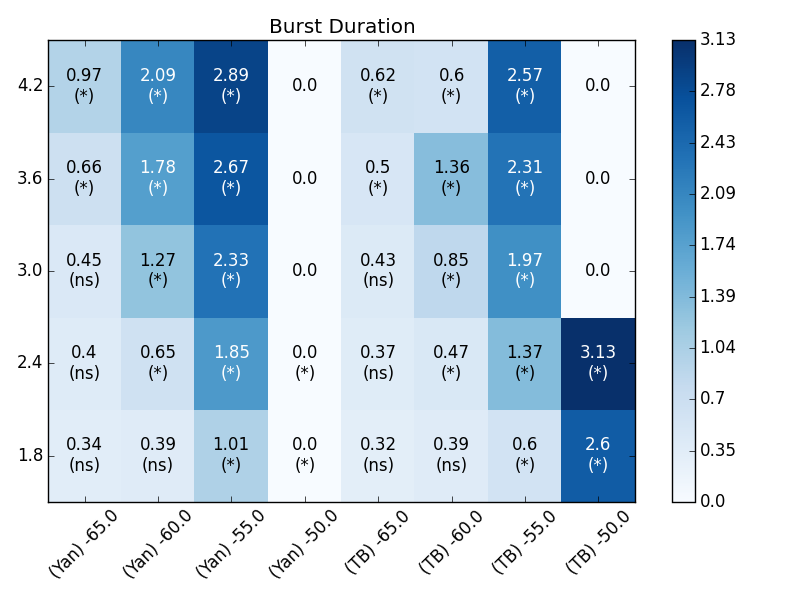
\includegraphics[scale=.4]{heatmap_Burst_Duration.png}
%	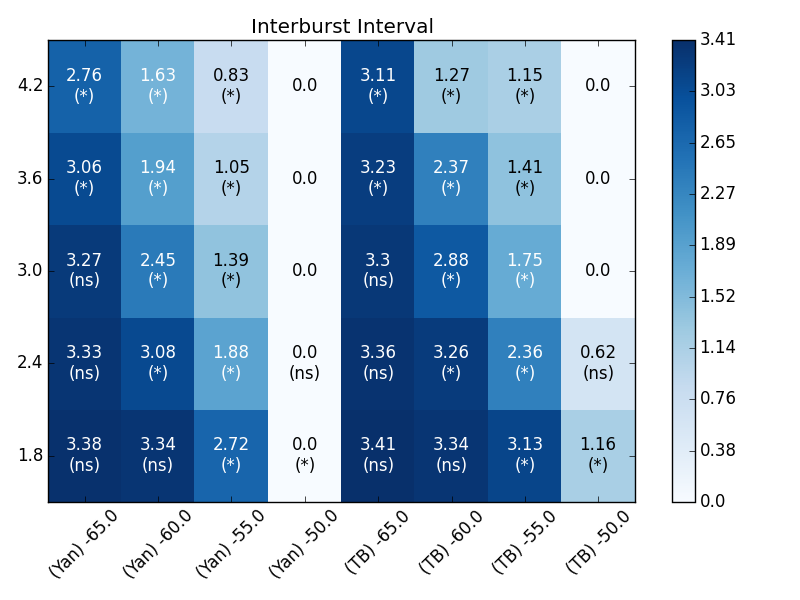
\includegraphics[scale=.4]{heatmap_Interburst_Interval.png}
%	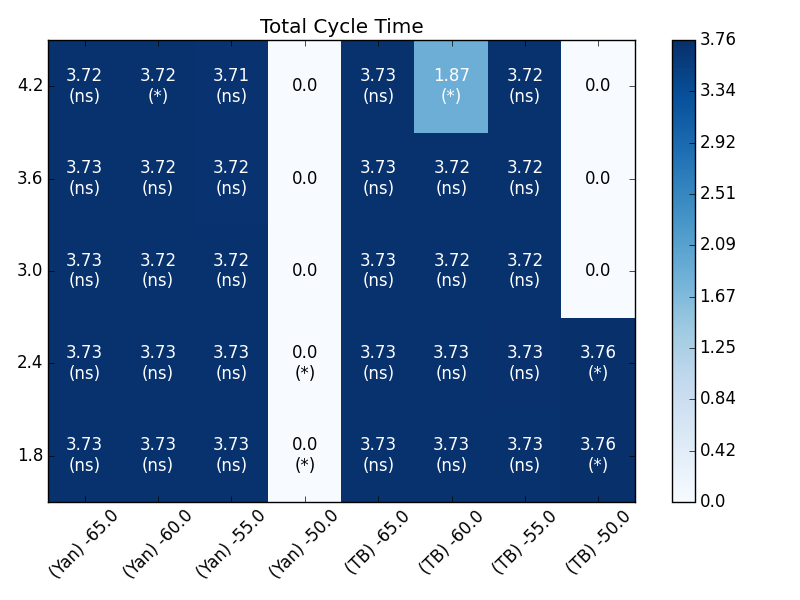
\includegraphics[scale=.4]{heatmap_Total_Cycle_Time.png}
%	\caption{Heat map showing variations in total cycle time with changes in $eL$, $g_{NaP}$, and model. Zeroes indicate  no bursting. Star (*) and (ns) symbols below each value indicates statistical significance between the corresponding cell for the other model.}
%	\label{fig:hmTCT}
%\end{figure}
%
% \begin{figure}[h]
%	\centering
%	\includegraphics[scale=\bcscale]{barchart_Burst_Duration.pdf}
%	\includegraphics[scale=\bcscale]{barchart_Interburst_Interval.pdf}
%	\caption{}
%	\label{fig:bcBD}
%\end{figure}


\subsection{Peak Variation}
Peak variations can be described by several measures, peaks per burst, intraburst frequency (the frequency of peaks within a burst), interpeak interval, and peak amplitude. The number of peaks per burst were increasingly model sensitive with increasing $eL$ and $g_{NaP}$. The Yan model consistently shows higher Peaks per Burst, except for $eL$=-60, where the TB model is significantly larger at $g_{NaP}$=3.0 and 3.6. Most comparisons between time series from the same model with different parameters show significant difference. Generally, PpB increased significantly with $eL$ and $g_{NaP}$, but PpB dropped significantly at $eL$ = -60 for TB  when $g_{NaP}$ = 4.2  and for Yan at $g_{NaP}$=3.6 and 4.2.


<Intraburst Frequency>
For smaller values of $eL$ (-65, -60) and higher values of $gnap$ (3.0, 3.6, and 4.2), TB had a significantly larger intraburst frequency than did Yan. The same occurred for small values of $gNaP$ (1.8, 2.4) at higher values of $eL$ (-55). Interestingly at $eL$ = -65 mV, the difference between the TB and Yan values decrease with decreasing $g_{NaP}$, but at $eL$=-60 the difference increased with decreasing $gnap$. No significant difference occurred between the models for low values of $eL$ at low values of $gnap$ or at high values of $eL$ with high values of $gnap$.

Intraburst frequency is significantly larger for the TB model at lower values of $eL$ and 

Average peak amplitude showed strong model-dependent significant differences(Figure~\ref{fig:hmPA}). However, no clear and consistent pattern of increase or decrease occurred, making it difficult to tell if peak amplitude was model-dependent in a meaningful way. Interpeak interval (not pictured) was not model dependent, as no statistically significant difference appeared between time series generated by different models with the same $eL$ and $g_{NaP}$ parameters.



%
%\begin{figure}[h]
%\centering
%	\subcaptionbox{Intraburst Frequency \label{fig:hmIF}}{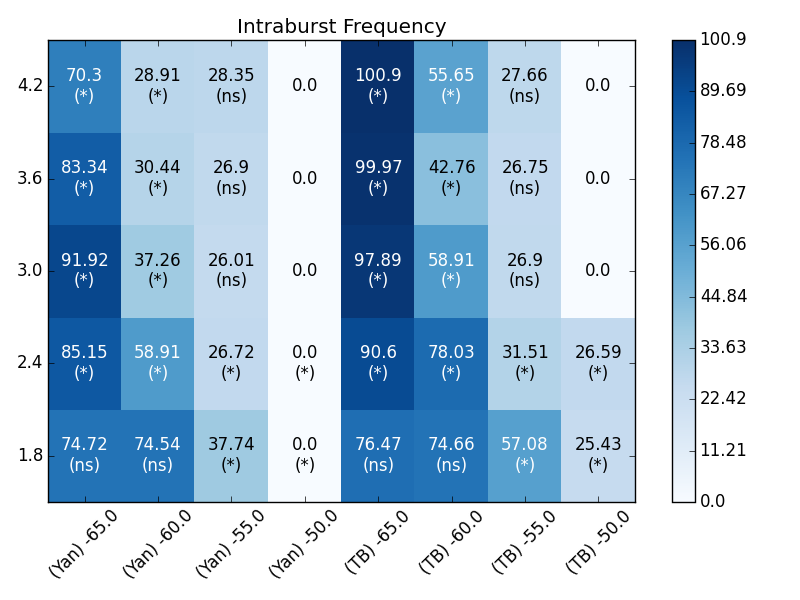
\includegraphics[scale=.4]{heatmap_Intraburst_Frequency.png}}%
%	\subcaptionbox{Peaks per Burst \label{fig:hmPpB}}{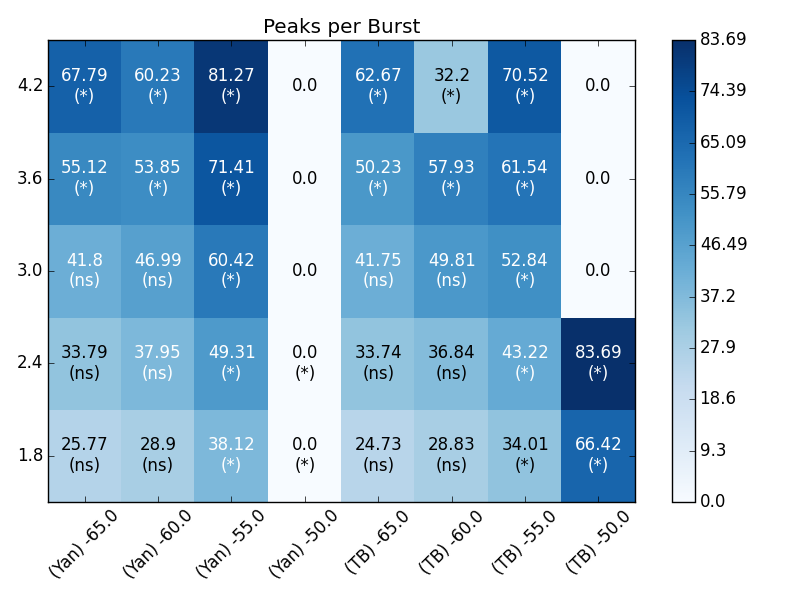
\includegraphics[scale=.4]{heatmap_Peaks_per_Burst.png}}%
%	\caption{}
%	\label{fig:hmPeakInBurst}
%\end{figure}
%\begin{figure}[h]
%	\centering
%	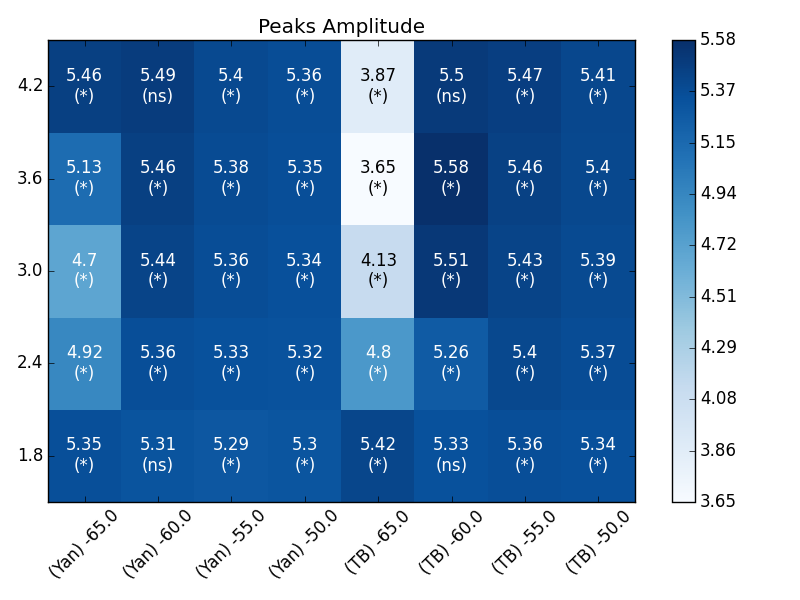
\includegraphics[scale=.4]{heatmap_Peaks_Amplitude.png}
%	\caption{Peak Amplitudes. Stars (*) indicate  which cells were significantly different from their other-model counterpart.}
%	\label{fig:hmPA}

%\end{figure}


%
\FloatBarrier
\section{Discussion}

We added the P2X7 model developed by Yan et al. to the somatic compartment of Toporikova and Butera's intrinsic bursting cell model and simulated the effects of changing $eL$ and $g_{NaP}$ on the activation (bursting?) patterns  in the generated time series. This was the first attempt to model an intrinsically bursting preBC neuron with a P2X component.

The uniformity of TCT suggests model and parameter insensitivity. It may be a characteristic of the TB model, for which burst duration and interburst interval appeared to asymptotically approach a value when eL and nap were [unpublished results]. It is interesting to note that the addition of the P2X7 component doesn't significantly effect this trend. Determining if this uniformity is due to the TB model could be tested by adding the P2X7 component to BRS model. 

Running BRS model singly and with the P2X7 component in the same parameter space would help further illuminate the effects of 
To locate the quiescent region, the parameter space needs to be extended. Primarily, the cell needs to be further depolarized by decreasing $eL$.
Additionally, testing more values within current parameter space  will help establish trends more securely.

A valid critique of the current study is that each run contains little more than 80 bursts, so longer simulation times might also be beneficial,  however, there was little variation of burst structure within a  majority of the time series, so this may be unnecessary.

<okay I'm running out of energy, so I'm resorting to bullet points. I'm not sure of the actual terminology>
-try to implement models of other P2XRs
-do isolated preBC neurons respond to ATP
-do preBC neurons respond to ATP when in the presence of astrocytes and/or microglia. How do they respond?
-Staining to find P2XRs on preBC neurons


\begin{figure}[h]
\includegraphics[scale=.25]{boxplot_Burst_Duration.pdf}
\includegraphics[scale=.25]{boxplot_Interburst_Interval.pdf}
\end{figure}
Also, P2X7 causes an influx of $Ca_{+2}$ which was not included in the TB+Yan model




PpB were probably parameter dependent within a model,


 
 
 \section{Abstract}
We extend the Toporikova-Butera model with a P2X7 model from [Yan] and compare their response to changes in $eL$ () and $g_{NaP}$ ().
We expect.....
We find...
Total cycle time was insensitive to changes in $eL$ and $g_{NaP}$ and model, while burst duration and interburst interval was sensitive to changes in all 3.
 
%\vspace{1.50cm}
%\noindent
\end{document}